%! Author = sudharsangopalakrishnan
%! Date = 6/18/21

% Preamble
\documentclass[11pt]{article}
\title{}
\author{Sudharsan Gopalakrishnan}
\date{April 1, 2021}

% Packages
\usepackage{amsmath}
\usepackage{xcolor}
\usepackage{graphicx}
\usepackage{hyperref}

% Document
\newcommand\mymaketitle{%
\begin{titlepage}
    \begin{center}
        \vspace*{\fill}
        {\LARGE \textbf{\textcolor{blue}{Get To Know GMOs}} \par}
        \vskip 1em {\Large Sudharsan Gopalakrishnan \par}
        \vskip 1em {\Large April 1, 2021 \par}

        \vspace*{\fill}
    \end{center}
    \small \centering This document was created using the \LaTeX{} programming language.
\end{titlepage}
}

\begin{document}
    \mymaketitle

    \newpage
    \section{Entry:}

    \paragraph{}
    Genetic engineering is used in several fields, predominantly Agriculture.
    Plants and other organisms that are genetically engineered are known as \textbf{Genetically
    Modified Organisms(GMOs)}, and this is such a trending topic today.
    GMOs are created by inserting desired genes into the target organism.
    Thousands of people currently debate whether
    they are beneficial or harmful to the environment and the society all around us.
    Countless negative allegations have been made, and some of them are based on concerns of human health.
    It is said that GMOs could trigger allergic reactions and bring side effects like toxicity, organ damage,
    or gene transfer.
    People even reported toxic effects caused by consuming GMOs. Other people claimed that
    genetically modified DNA is unstable and that GMO consumers’ health would be damaged.
    To confirm this, scientists use mutagenesis, or the creation of random mutations, to test if food products or drugs cause
    high mutation rates.
    Along with other methods of testing, however, many of them concluded that GMOs are not
    mutagenic crops, meaning that they do not cause mutations within the consumers.
    \paragraph{}
    While many people either use their current research or instincts to make claims whether GMOs are good or bad,
    there really is no evidence to prove any side.
    No one really knows if GMOs are good or bad.
    However, there are some already known proven facts about GMOs, particularly on their good side.
    GMOs are advantaged over other crops as they generally have \textbf{resistance} against insects, drought, and diseases.
    Many GMOs are even herbicide tolerant, meaning that farmers can easily fight weeds or other unwanted plants on their farms without harming important plants and vegetation.
    Some other benefits of GMOs are increased crop yields, enhanced nutrition and food quality, and better food security.
    They are also generally less costly than normal food because of the reduction of pesticide use.
    GMOs made for insect resistance
    generally use the Bt gene, which can be extracted from a bacterium known as Bacillus Thuringiensis which provides natural insect
    resistance.
    This makes it much easier for farmers to plant GMOs as opposed to farming normal organic crops.
    Furthermore, GMO crops have positively impacted the world by reducing tillage and fuel use, decreasing greenhouse gas emissions.
    The FDA as well as the USDA even approve that GMOs are safe.
    GMOs have helped feed the needy and the malnutritious populations all around the world.
    And as GMO crops are increasingly accepted, we are sure to see more positive environmental impacts in the future such as less waste due to new varieties of produce.
    \paragraph{}
    Right now, in the United States, there are currently a few types of GMOs: corn, soybean, cotton, alfalfa, sugar beet, apple, squash and papaya.
    Despite approval and confirmations that GMOs are safe, people still tend to avoid them.
    And this gets increasingly difficult as time passes since GMOs are dominating today’s supermarkets and grocery stores in the world.
    The main problem here is \textbf{mislabeling}.
    People generally look at labels of food when buying them in stores and might be misled.
    Companies and brands often like to label their products in a way that would seem appealing to consumers, no matter the ingredients.
    For example, products that are labeled “organic” are probably not completely organic and may use some GMOs. That being said, this only applies to food products that are not labeled “100 percent organic” instead of just “organic”.
    Labels like these can be extremely vague, and this is primarily due to non stringent regulations, especially in the United States.
    So, how can we minimize misunderstandings of labels?
    Well, as a consumer myself and an avid science student, it is very important for people to first learn the science around biotechnology and genetic engineering of organisms and plants and then make decisions based on food choice and understanding to facilitate reading labels.
    And I started doing my part to educate my community by initiating conversations with family, friends, and neighbors about their food choices on labels and sharing the science behind labels to help them make their own informed decisions with regard to buying food products.
    I hope my efforts will one day positively impact my community.

    \newpage

    \section{References:}
    \begin{itemize}
        \item[] Norris, Megan L. “Will GMOs Hurt My Body?
        The Public’s Concerns and How Scientists Have Addressed Them.” Sitn,
        Harvard University, 10 August 2015, https://sitn.hms.harvard.edu/flash/2015/will-gmos-hurt-my-body/.
        \item[] Phillips, Theresa.
        “Genetically Modified Organisms (GMOs): Transgenic Crops and Recombinant DNA Technology.” Nature Education,
        Nature Education, 2008, https://www.nature.com/scitable/topicpage/genetically-modified-organisms-gmos-transgenic-crops-and-732/.
        \item[] Raman, Ryan.
        “GMOs: Pros and Cons, Backed by Evidence.” Healthline, Healthline, 2 July 2020, https://www.healthline.com/nutrition/gmo-pros-and-cons#definition.
    \end{itemize}

    \section{Key words:}
    \begin{itemize}
        \item Genetically Modified Organisms(GMOs)
        \item Resistance
        \item Mislabeling
    \end{itemize}

    \newpage
    \section{Image:}
    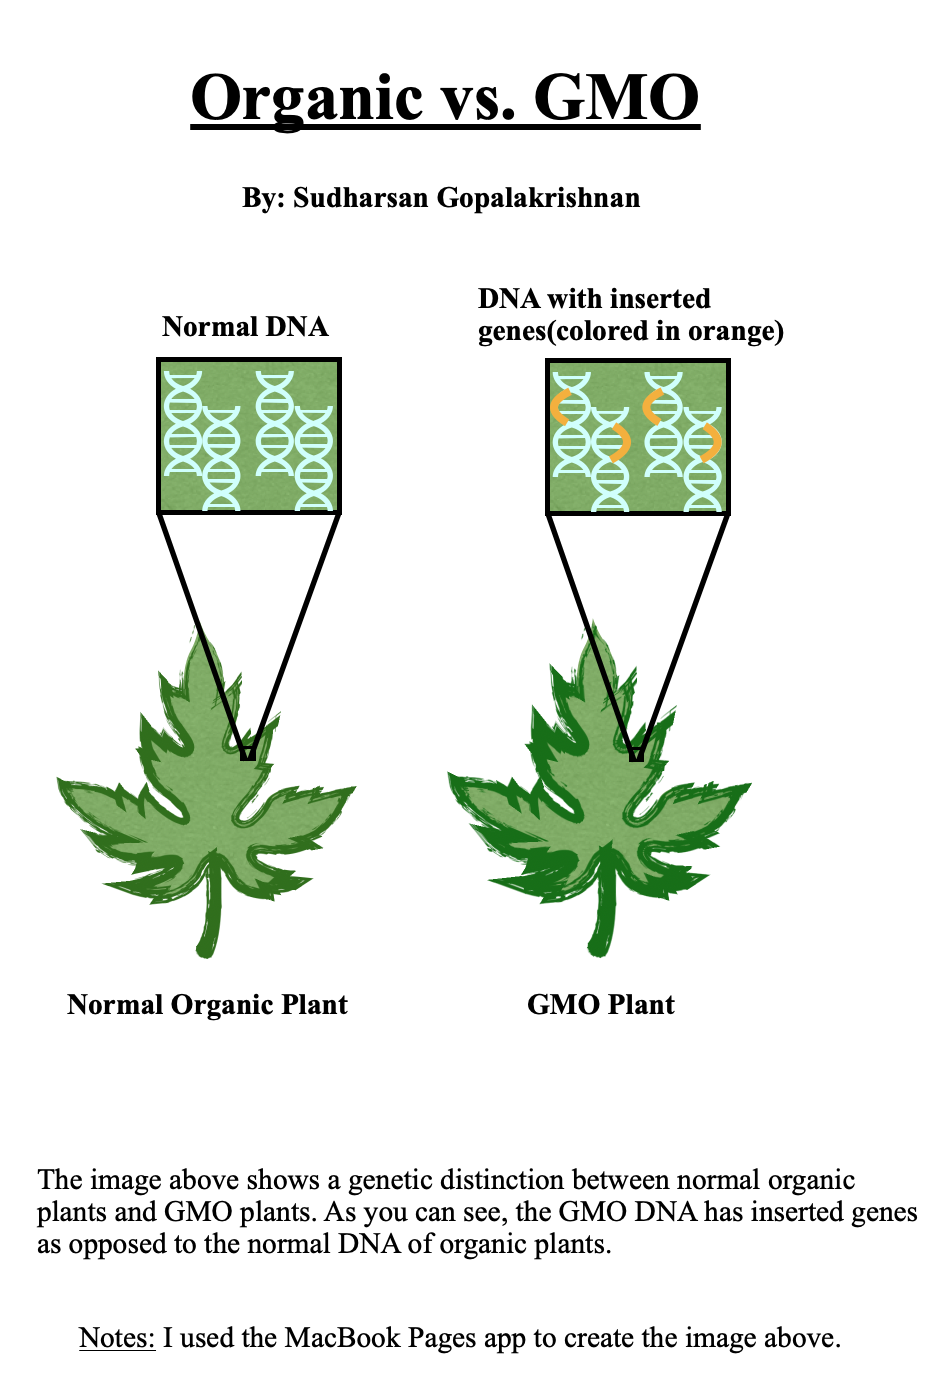
\includegraphics[width=350]{Sudharsan Gopalakrishnan Image.jpg}

    \section{My Independent GMO Outreach Efforts}
    The links to my website, my Facebook page, and my Youtube channel are right below.
    They all comprise my independent research on GMOs.

    \textbf{Links:}
    \begin{itemize}
        \item \textcolor{blue}{\href{https://www.reach2sudharsan.com/independent-research--gmo.html}{GMO Community Outreach}}
        \item \textcolor{blue}{\href{https://www.facebook.com/National-4-H-Science-Matters-Project-Get-to-know-GMOs-112058317207683/?view_public_for=112058317207683}{Facebook Page}}
        \item \textcolor{blue}{\href{https://www.youtube.com/channel/UCbFpUuam0C-5Ge0Y3BrbvLw/videos?app=desktop}{Youtube Channel}}
    \end{itemize}


\end{document}